\begin{figure}[h]
  \centering
  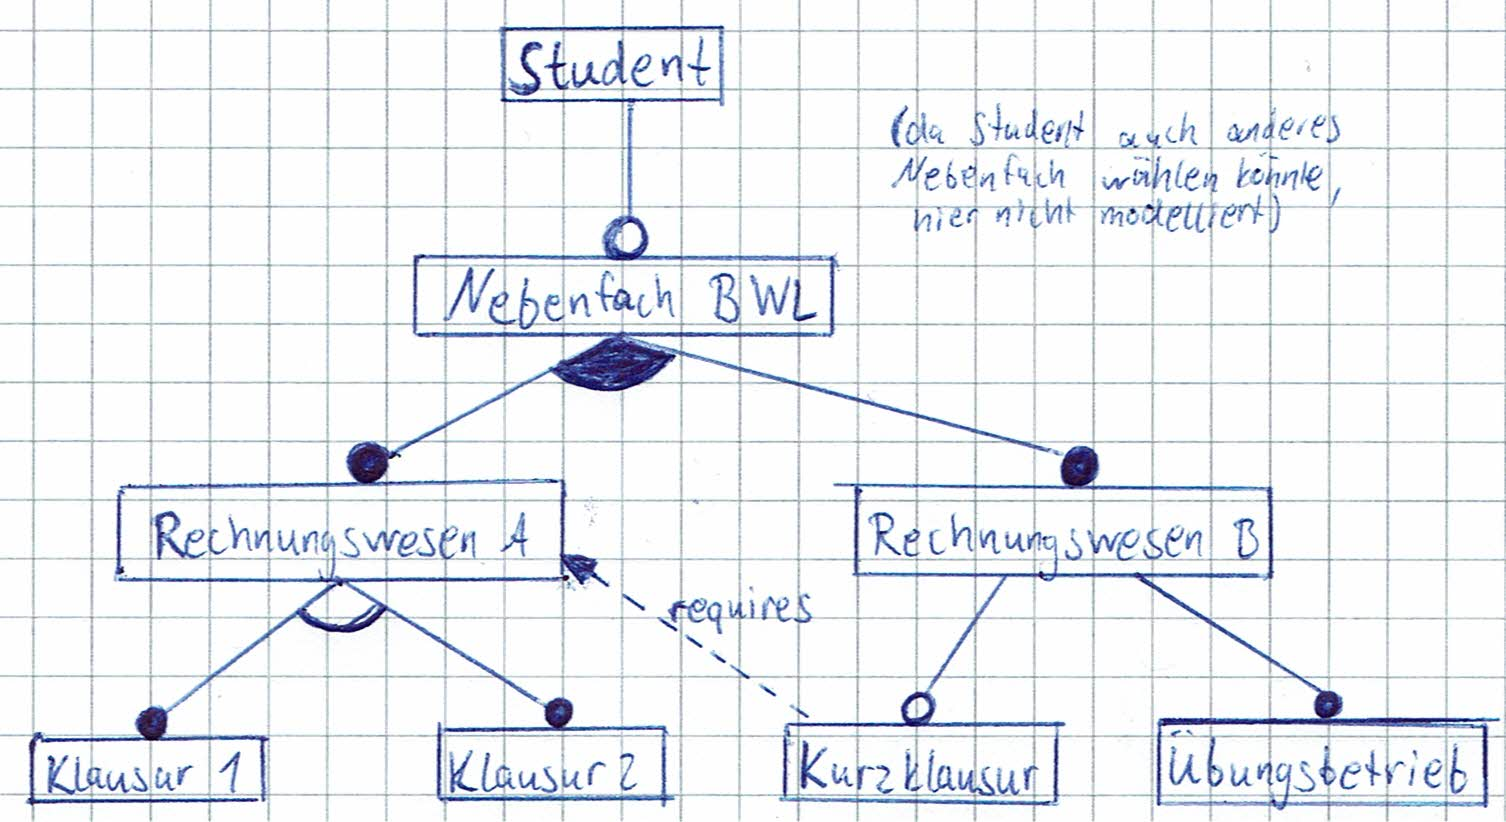
\includegraphics{1_featdiag}
\end{figure}

Nun folgen alle 8 erlaubten Konfigurationen. Es wurden folgende Abkürzungen benutzt:
\begin{itemize}
\item Nebenfach BWL $\mapsto$ BWL
\item Rechnungswesen A(B) $\mapsto$ RW A(B)
\item Klausur 1(2) $\mapsto$ KL 1(2)
\item Kurzklausur $\mapsto$ KKL
\item Übungsbetrieb $\mapsto$ Übung
\end{itemize}

\begin{figure}[h]
  \centering
  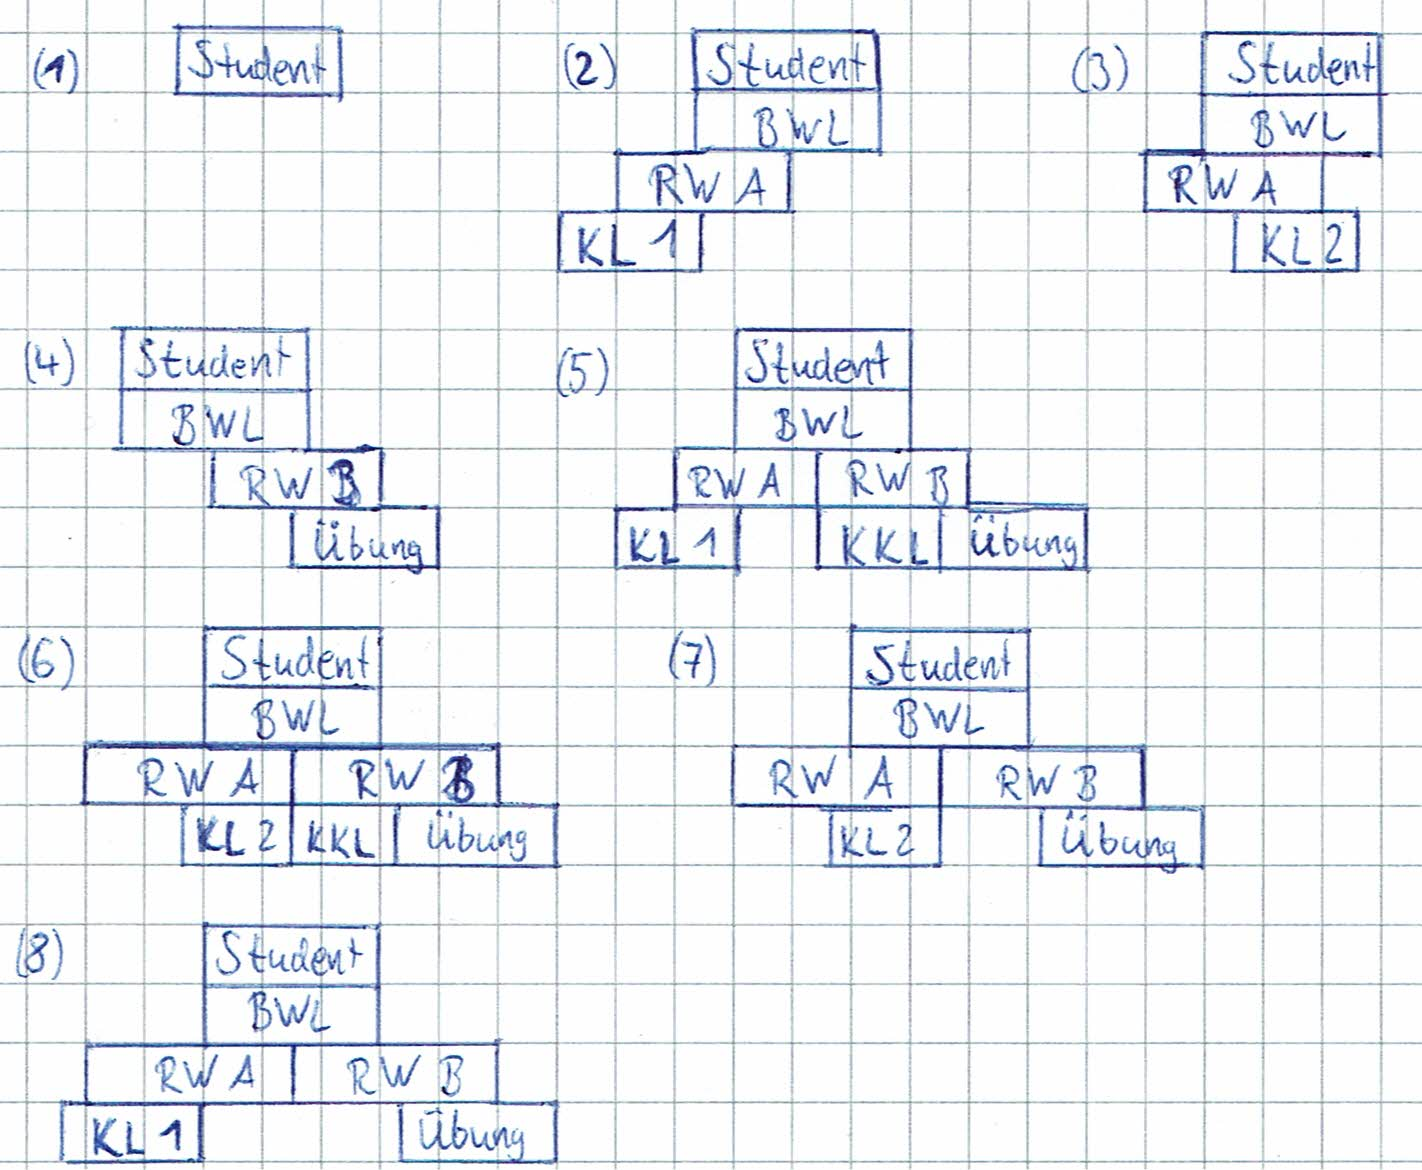
\includegraphics{1_config}
\end{figure}